%%%%%%%%%%%%%%%%%%%%%%%%%%%%%%%%%%%%%%%%%%%%%%%%%%%%%%%%%%%%%%%%%%%%%%%
%%%%%%%%%%%%%%%%%%%%%%%%%%%%%%%%%%%%%%%%%%%%%%%%%%%%%%%%%%%%%%%%%%%%%%%
%%%%%                                                                 %
%%%%%     <file_name>.tex                                             %
%%%%%                                                                 %
%%%%% Author:      <author>                                           %
%%%%% Created:     <date>                                             %
%%%%% Description: <description>                                      %
%%%%%                                                                 %
%%%%%%%%%%%%%%%%%%%%%%%%%%%%%%%%%%%%%%%%%%%%%%%%%%%%%%%%%%%%%%%%%%%%%%%
%%%%%%%%%%%%%%%%%%%%%%%%%%%%%%%%%%%%%%%%%%%%%%%%%%%%%%%%%%%%%%%%%%%%%%%


\chapter{Experimental Results}

\section{Performance Evaluation}

\subsection{Logging and SD-card driver} \label{logging_perf}

Experimental evaluation of the SD-card driver by visualizing write operations using an oscilloscope attached to the SPI bus revealed an important trade-off that greatly impacts the performance of the logging driver. Although many overheads are introduced by the FAT file system, the SD card also introduces a overhead during read and write operations. As write operations are more relevant in this particular application the following will examine only write operations.

Figure~\ref{fig:sd_card_write} illustrates the initial steps of writing to an SD-card. First a write command is issued. This is then followed by one or more data packets consisting of a data token, 1-2048 bytes of data and two CRC bytes. Between the cursors in Figure~\ref{fig:sd_card_write} one data packet is transmitted. Once all the data packets have been transmitted, a write termination command is transmitted. This last command is omitted if a single block write operation is used.

\begin{figure}[H]
    \centering \includegraphics[width=1.0\textwidth]{./figures/"SPI SD WRITE".PNG}
    \caption{Write command and data packet on SPI bus with SD card.}
    \label{fig:sd_card_write}
\end{figure}

Between each data packet and after the full sequence of commands and packets, the SD card enters a busy state where it is processing the written data. As Figure~\ref{fig:sd_card_write_wait} shows, the busy time after the full sequence (or rather after the write termination command) is particularly long in relation to the transmission time of a single data packet.

\begin{figure}[H]
    \centering \includegraphics[width=1.0\textwidth]{./figures/"SPI SD WRITE1".PNG}
    \caption{Wait time after writing data packet to SD card.}
    \label{fig:sd_card_write_wait}
\end{figure}

Further testing revealed that, while the busy time between data packets is very small, the busy time is almost completely dominated by the busy time at the end of a write operation. This is further verified by another test where chunks of different sizes are repeatedly written to a file in the FAT file system and the data rate observed. Table~\ref{tab:write_speed} shows the results of this test. As can be seen from Figure~\ref{fig:write_speed} the write speed behaves almost linearly compared to the chunk size.

\begin{table}[htbp]
    \caption{Write speeds for chunks of different sizes.}
    \label{tab:write_speed}
    \centering\begin{tabular}{@{}lcr@{}} \toprule
    \textbf{Chunk size} & \textbf{Average data-rate} \\ \midrule
        256 bytes & 21 kB/s \\
        512 bytes & 41 kB/s \\
        1024 bytes & 80 kB/s \\
        2048 bytes & 148 kB/s \\
        4096 bytes & 254 kB/s \\ \bottomrule
    \end{tabular}
\end{table}

\begin{figure}[H]
\centering
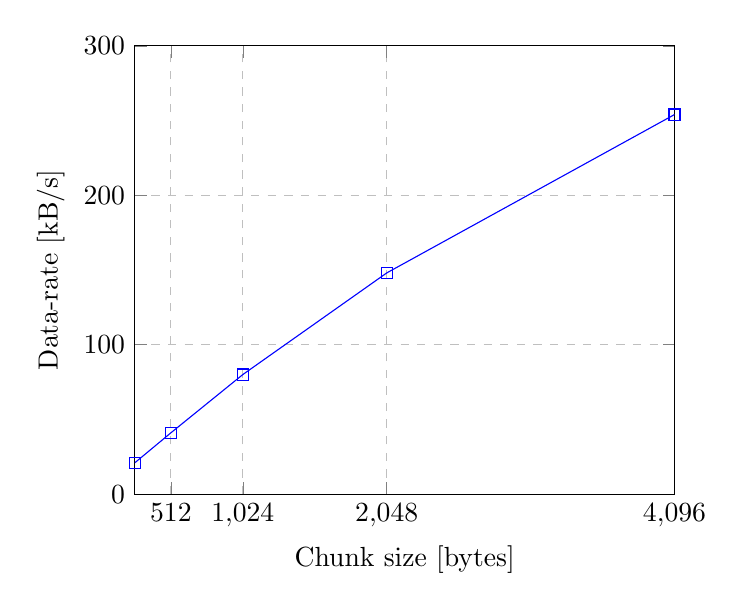
\begin{tikzpicture}
\begin{axis}[
    xlabel={Chunk size [bytes]},
    ylabel={Data-rate [kB/s]},
    xmin=256, xmax=4096,
    ymin=0, ymax=300,
    xtick={512,1024,2048,4096},
    xmajorgrids=true,
    ymajorgrids=true,
    grid style=dashed,
]
 
\addplot[
    color=blue,
    mark=square,
    ]
    coordinates {
    (256,21)(512,41)(1024,80)(2048,148)(4096,254)
    };
 
\end{axis}
\end{tikzpicture}
\caption{Write speeds for chunks of different sizes.}
\label{fig:write_speed}
\end{figure}

Given these results we have a memory/data-rate trade-off. Memory is limited on the micro-controller but we also want to maximize the amount of data that can be logged. In-field experimentation showed that under most circumstances write buffers of 2048 bytes are sufficient to achieve the data-rate necessary to log all sensor data. Nonetheless, we ended up using buffers of 4096 bytes to insure that no data would be lost.

\subsubsection{Comparison to Escher}

\todo{DO THIS}

\subsection{Networking}

Using an oscilloscope the SPI bus with the micro-controller and Ethernet controller can be monitored. Figures ~\ref{fig:net_send} and ~\ref{fig:net_recv} visualize the sequence of commands necessary for sending and receiving short 12 byte network packets. In order to send a packet, the micro-controller must first read the write pointer it should use from the Ethernet controller. Then it can write to the Ethernet controller's packet RAM at the read address. It must then update the write pointer so the Ethernet controller knows the length of the packet and finally confirm the packet using a send command. The sequence for receiving packets is analogous. Notice however, that the process is triggered by the interrupt signal from the Ethernet controller.

\begin{figure}[H]
    \centering \includegraphics[width=1.0\textwidth]{./figures/"SPI NET SEND".PNG}
    \caption{Command sequence for sending a network packet on SPI bus.}
    \label{fig:net_send}
\end{figure}

From Figure~\ref{fig:net_send} we can see that it takes only 39 microseconds to complete all commands necessary to send a network packet of this size at maximum clock rate supported by the SPI interface (12,5 MHz). The use of the DMA controller leads to uninterrupted transmission of each command on the bus. Although the demonstrated performance this is more than fast enough for this application, the driver could still be optimized to reduce the time between commands. Some of the computation necessary for the next command is performed after the previous command is transmitted. Although this would increase memory usage, it could be performed while the previous command is still transmitting. On the other hand, for longer packets the time is dominated by the transmission subsequence labelled "write packet" in Figure~\ref{fig:net_send}.

The same optimization could be applied to the reception of network packets but again Figure~\ref{fig:net_recv} shows that the full sequence only takes 47 microseconds, which is sufficient for this application. 

\begin{figure}[H]
    \centering \includegraphics[width=1.0\textwidth]{./figures/"SPI NET RECV".PNG}
    \caption{Command sequence for receiving a network packet on SPI bus.}
    \label{fig:net_recv}
\end{figure}

\todo{Maybe mention delay hack?}

\section{In-Field Evaluation: Competition}




\section{Conclusion}

Summary of work

What I did

Quantitative data

How it was used in the real world

\section{Outlook}